\documentclass[a4paper, 12pt]{article}
\usepackage{amssymb}
\usepackage[english,italian]{babel}
\usepackage{xspace}
\usepackage{tikz}
\usepackage[newitem,newenum,neverdecrease]{paralist}
\usepackage{amsmath,amssymb,amsfonts,mathrsfs,latexsym,stmaryrd}
\usepackage{mathtools}
\usepackage{amsthm}
\usepackage{ifpdf}
\usepackage{cases}
\usepackage{listings}
\usepackage{bm}
\usepackage{titlesec}
\usepackage[T1]{fontenc}
\usepackage[utf8]{inputenc}
\usepackage{xcolor}
\usepackage{colortbl}
\usepackage{makecell}
\usepackage{geometry}
\usepackage{layout}
\usepackage{eurosym}
\usepackage{wrapfig}
\usepackage{hyperref}

\begin{document}
	
	% interlinea 1
	\linespread{1}
	
	% 2.5cm di margine su ogni lato
	\newgeometry{
		top=2.5cm,
		bottom=2.5cm,
		left=2.5cm,
		right=2.5cm
	}
	
	% --- COPERTINA ---
	\vspace{4cm}
	\begin{center}
		\includegraphics[width=0.65\textwidth]{Images/LogoGIP.png}\\
		{\Huge NOME}\\
		\vspace{0.5cm}
		{\large Sottotitolo}\\
		\vspace{1cm}
		A cura di:
	\end{center}
	\newpage
	
	% indice
	\tableofcontents
	\newpage
	
	\section{Executive Summary}
	\newpage
	\section{Problema da risolvere}
	Ai giorni nostri sempre maggiore importanza viene attribuita alle fonti di energia rinnovabili. Tra queste, l'energia solare è particolarmente degna di nota in quanto inesauribile, disponibile in enormi quantità nonché utilizzabile per produrre energia elettrica e termica.\\
	I dispositivi in grado di sfruttare tale risorsa sono i pannelli fotovoltaici e i solari termici. Impianti che sfruttano queste tecnologia sono diffusi in tutto il mondo e vengono installati in notevoli quantità sia da grandi imprese che da utenti privati. Sono diversi i vantaggi forniti dagli impianti fotovoltaici: oltre a ridurre l'inquinamento, non utilizzando combustibili fossili, permettono di godere di sgravi fiscali fino all'80\% sulle imposte andando a produrre autonomamente energia, non dovendo attingere dalla rete elettrica nazionale.\\\\
	Nel momento in cui si decide di installare un impianto fotovoltaico, si deve tenere presente non solo del costo della installazione effettiva ma anche di quello della manutenzione dell'apparecchio durante la vita dell'impianto stesso dato che ogni pannello fotovoltaico ha un tempo di vita nominale oltre il quale perde la capacità di produrre energia. La quasi totalità di questo costo di manutenzione è relativo alla pulizia del pannello: operazione fondamentale per preservare il corretto funzionamento dell'impianto.\\
	In assenza di adeguata pulizia non solo il pannello fotovoltaico si deteriora più rapidamente ma cala la sua efficienza energetica. La sporcizia che va a depositarsi sulla superficie fotovoltaica riduce la quantità di radiazioni solari ricevute e di conseguenza anche la quantità di energia prodotta, andando a diminuire il ritorno economico, tanto che un pannello fotovoltaico sporco può arrivare ad una perdita di prestazioni fino al 30\% dell'intero impianto. Inoltre, a seconda della locazione in cui sono posizionati i pannelli, questi possono dover essere puliti più o meno frequentemente.\\
	La superficie può venire sporcata da diversi fattori: tra i più comuni vi sono piogge acide, polveri e smog, ma anche foglie, guano e sabbia. Nella figura di seguito si mostra un esempio di impianto particolarmente sporco:
	\begin{figure}[h]
		\centering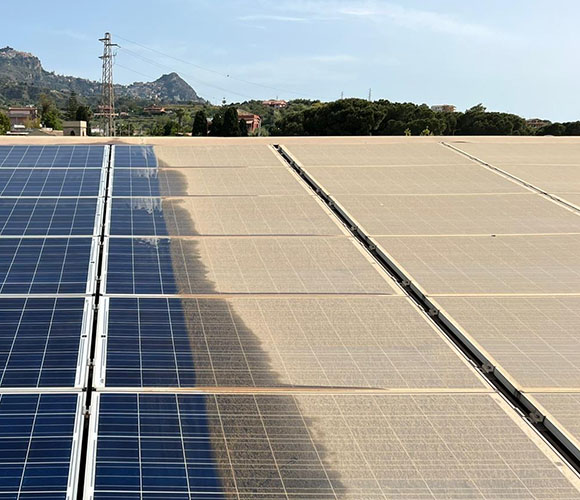
\includegraphics[width=0.5\textwidth]{Images/pannelli_sporchi2.jpg}
	\end{figure}\\
	Per affrontare il problema della pulizia, il proprietario dell'impianto può scegliere se rivolgersi ad imprese specializzate che effettuano pulizia a domicilio oppure prevenire il problema scegliendo di installare pannelli autopulenti di ultima generazione. Entrambe queste soluzioni hanno però dei limiti: per quanto riguarda la prima possibilità è l'utente stesso che deve accorgersi di quando sopraggiunge il momento opportuno per eseguire la pulizia e deve mobilitarsi per contattare l'impresa adeguata per un costo che in media varia tra i 100\euro e 300\euro.\\
	Parlando invece di pannelli autopulenti essi sono un arma a doppio taglio.\\
 Possono essere realizzati sfruttando diverse tecnologie che spaziano dall'impiego di materiali con attrito estremamente ridotto sfruttando l'acqua piovana per lavare via la sporcizia, all'uso di impulsi elettrici per far letteralmente "saltare via" le impurità dalla superficie. Tuttavia, mentre queste tecnologie di ultimissima generazione sono fuori dalla portata dei molti, l'uso di materiali dall'attrito ridotto (oltre che essere caratterizzati da costi di acquisto superiori rispetto  a pannelli tradizionali) comporta una forte dipendenza dalle precipitazioni atmosferiche che, per di più, possono anche risultare controproducenti dal momento che in aree cittadine, o generalmente più inquinate, l'acqua piovana andrebbe a depositare ulteriori detriti sulla superficie.\\
	\section{Soluzione proposta}
	La nostra proposta consiste nel fornire un sistema completamente automatizzato per la pulizia dell'impianto fotovoltaico. L'idea di base è quella di monitorare costantemente l'efficienza energetica di ogni pannello in modo tale da rendersi conto quando non è più in grado di fornire adeguate prestazioni a causa dello sporco che vi si è depositato sopra. Quando l'efficienza scende sotto una certa soglia prestabilita dal proprietario; il nostro sistema è in grado di effettuare la pulizia usando l'adeguato detergente, reso disponibile in una piccola cisterna installata nello stabile, rilasciandolo sul pannello.\\
	% immagine dell'impianto
	Questa soluzione consentirebbe al proprietario dell'impianto di risparmiare notevolmente sul costo della pulizia e sul tempo da dedicarvi, in quanto questa verrebbe effettuata automaticamente dal sistema senza che l'utente debba preoccuparsi di controllare l'impianto.\\
	Il liquido adeguato per la pulizia della superficie è l'acqua osmotica, o osmotizzata, che può assere acquistata dall'utente al costo di circa 1 \euro/L in modo che egli possa occuparsi di mantenere attivo il sistema in completa autonomia, senza dover contattare un tecnico o un'impresa specializzata.\\
	\begin{wrapfloat}{figure}{r}{0pt}
		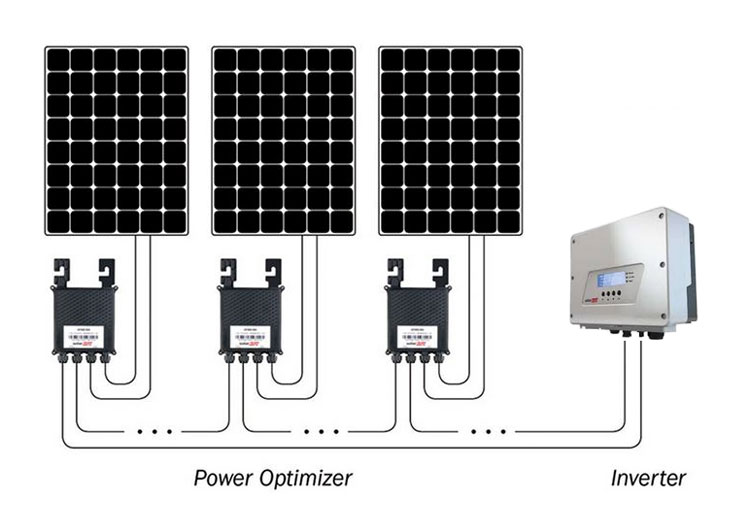
\includegraphics[width=0.5\textwidth]{Images/ottimizzatori.jpg}
	\end{wrapfloat}
	La misurazione dell'efficienza energetica è realizzabile in modo relativamente semplice. Il nostro dispositivo dialoga direttamente con gli ottimizzatori: delle componenti già presenti all'interno dell'impianto fotovoltaico, che a intervalli di tempo regolari raccolgono i report provenienti dai vari pannelli. Ciascun report contiene, tra le altre informazioni, l'efficienza energetica che può essere intercettata dal nostro dispositivo che ne tiene traccia. Questo metodo di misurazione è efficace poiché, invece di sfruttare l'energia prodotta (che può variare a seconda delle condizioni atmosferiche) si basa sull'efficienza, che esprime il rapporto tra l'energia generata e l'energia solare ricevuta. Qualora il valore dovesse diminuire significherebbe che le prestazioni del pannello stanno calando e il sistema si occuperà di rilasciare il detergente sulla superficie.
	\section{Il settore}
	% https://sonnen.it/crescita-del-fotovoltaico-2023-il-boom-e-reale/ --> ho preso tanto da qua
	% https://www.lumi4innovation.it/accumulo-energia-rinnovabili-energy-storage/
	\emph{Osmos} vuole inserirsi all'interno del settore fotovoltaico, avendo lo scopo di rendere più utili e performanti queste fonti sostenibili.\\\\
	Grazie alla sempre maggiore spinta internazionale verso le fonti di energia rinnovabili, il settore fotovoltaico è in notevole espansione nel mondo.\\
	Importante è anche la crescita della capacità fotovoltaica installata in Italia. Nei primi sette mesi del 2023, in Italia, sono stati installati oltre 2,7 GW, con una crescita del 113\% rispetto allo stesso periodo dell'anno precedente e con un importante contributo degli impianti residenziali (circa il 47\% della capacità totale connessa).\\\\
	Secondo i dati forniti da \href{https://www.terna.it/it/sistema-elettrico/dispacciamento/fonti-rinnovabili}{\emph{Gaudì}}, la potenza fotovoltaica cumulata in Italia, ad agosto 2023, ha superato i 28 GW con oltre 1,4 milioni di installazioni attive. Un dato notevole se si considera che nei primi otto mesi dell'anno sono stati installati 3.123 MW di potenza fotovoltaica con andamenti diversi per i vari segmenti:
	\begin{itemize}
		\item residenziale (impianti sotto i 12 kW) ha registrato l'installazione di 1.379 MW;
		\item commerciale ed industriale (impianti tra i 20 kW e 1 MW) registrati 1.088 MW;
		\item utility-scale (impianti con potenza superiore a 1 MW) aumento di 426 MW.
	\end{itemize}
	I dati registrati dal settore del fotovoltaico e le previsioni di crescita, mostrate nelle figure di seguito, sottolineano il ruolo centrale delle rinnovabili nel percorso di transizione energetica globale, riportando un indice CAGR che si attesta intorno al 30\%.
	\begin{center}
		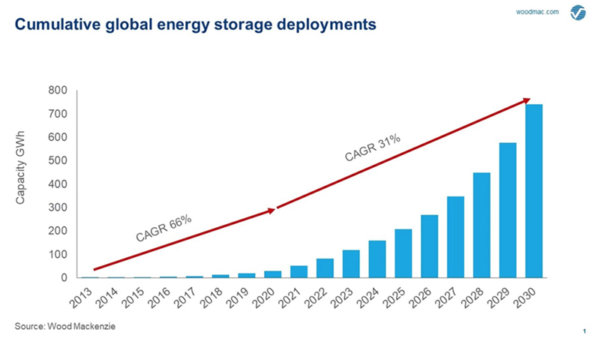
\includegraphics[width=0.73\textwidth]{Images/previsioni_solare.jpg}
		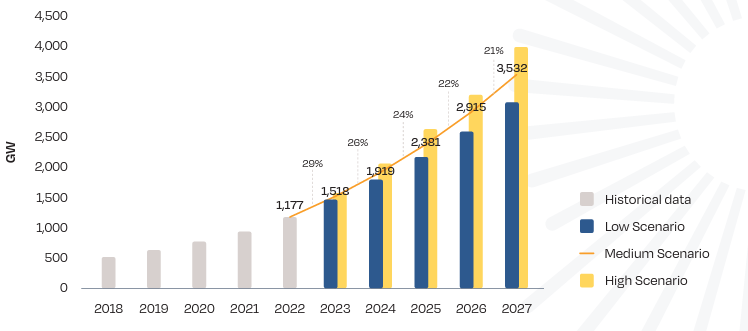
\includegraphics[width=0.73\textwidth]{Images/andamento_pannelli2.png}
	\end{center}
	Il settore del fotovoltaico è sufficientemente vasto da poter essere a sua volta suddiviso in due parti: una prima parte che comprende le imprese produttrici di moduli fotovoltaici (in cui i principali attori sono \emph{Sunpower, Panasonic, Exe Solar} e simili) e una seconda parte che riguarda le imprese produttrici di componenti cooperanti coi moduli fotovoltaici.\\\\
	Sebbene esistano enti che si pongono a cavallo di questa partizione, \emph{Osmos} fa capo solamente alla seconda categoria. All'interno di questa non vi è grande frammentazione, infatti la maggioranza è occupata da \emph{Abb Spa}: una società fortemente coinvolta nella produzione di apparecchiature che garantiscono continuità di servizio, affidabilità e ritorno dell'investimento tramite interruttori, dispositivi di misurazione, sensori e altro.\\
	I prodotti e servizi forniti da \emph{Abb Spa} sono poi utilizzabili anche in moltissimi altri settori eterogenei; questo aumenta considerevolmente l'influenza e il potere economico dell'impresa stessa, dandole la possibilità di imporsi nei confronti di altre società più specializzate quali \emph{Enel X} e \emph{SoralEdge Tecnology} come riportato nel grafico seguente:\\
	\begin{center}
		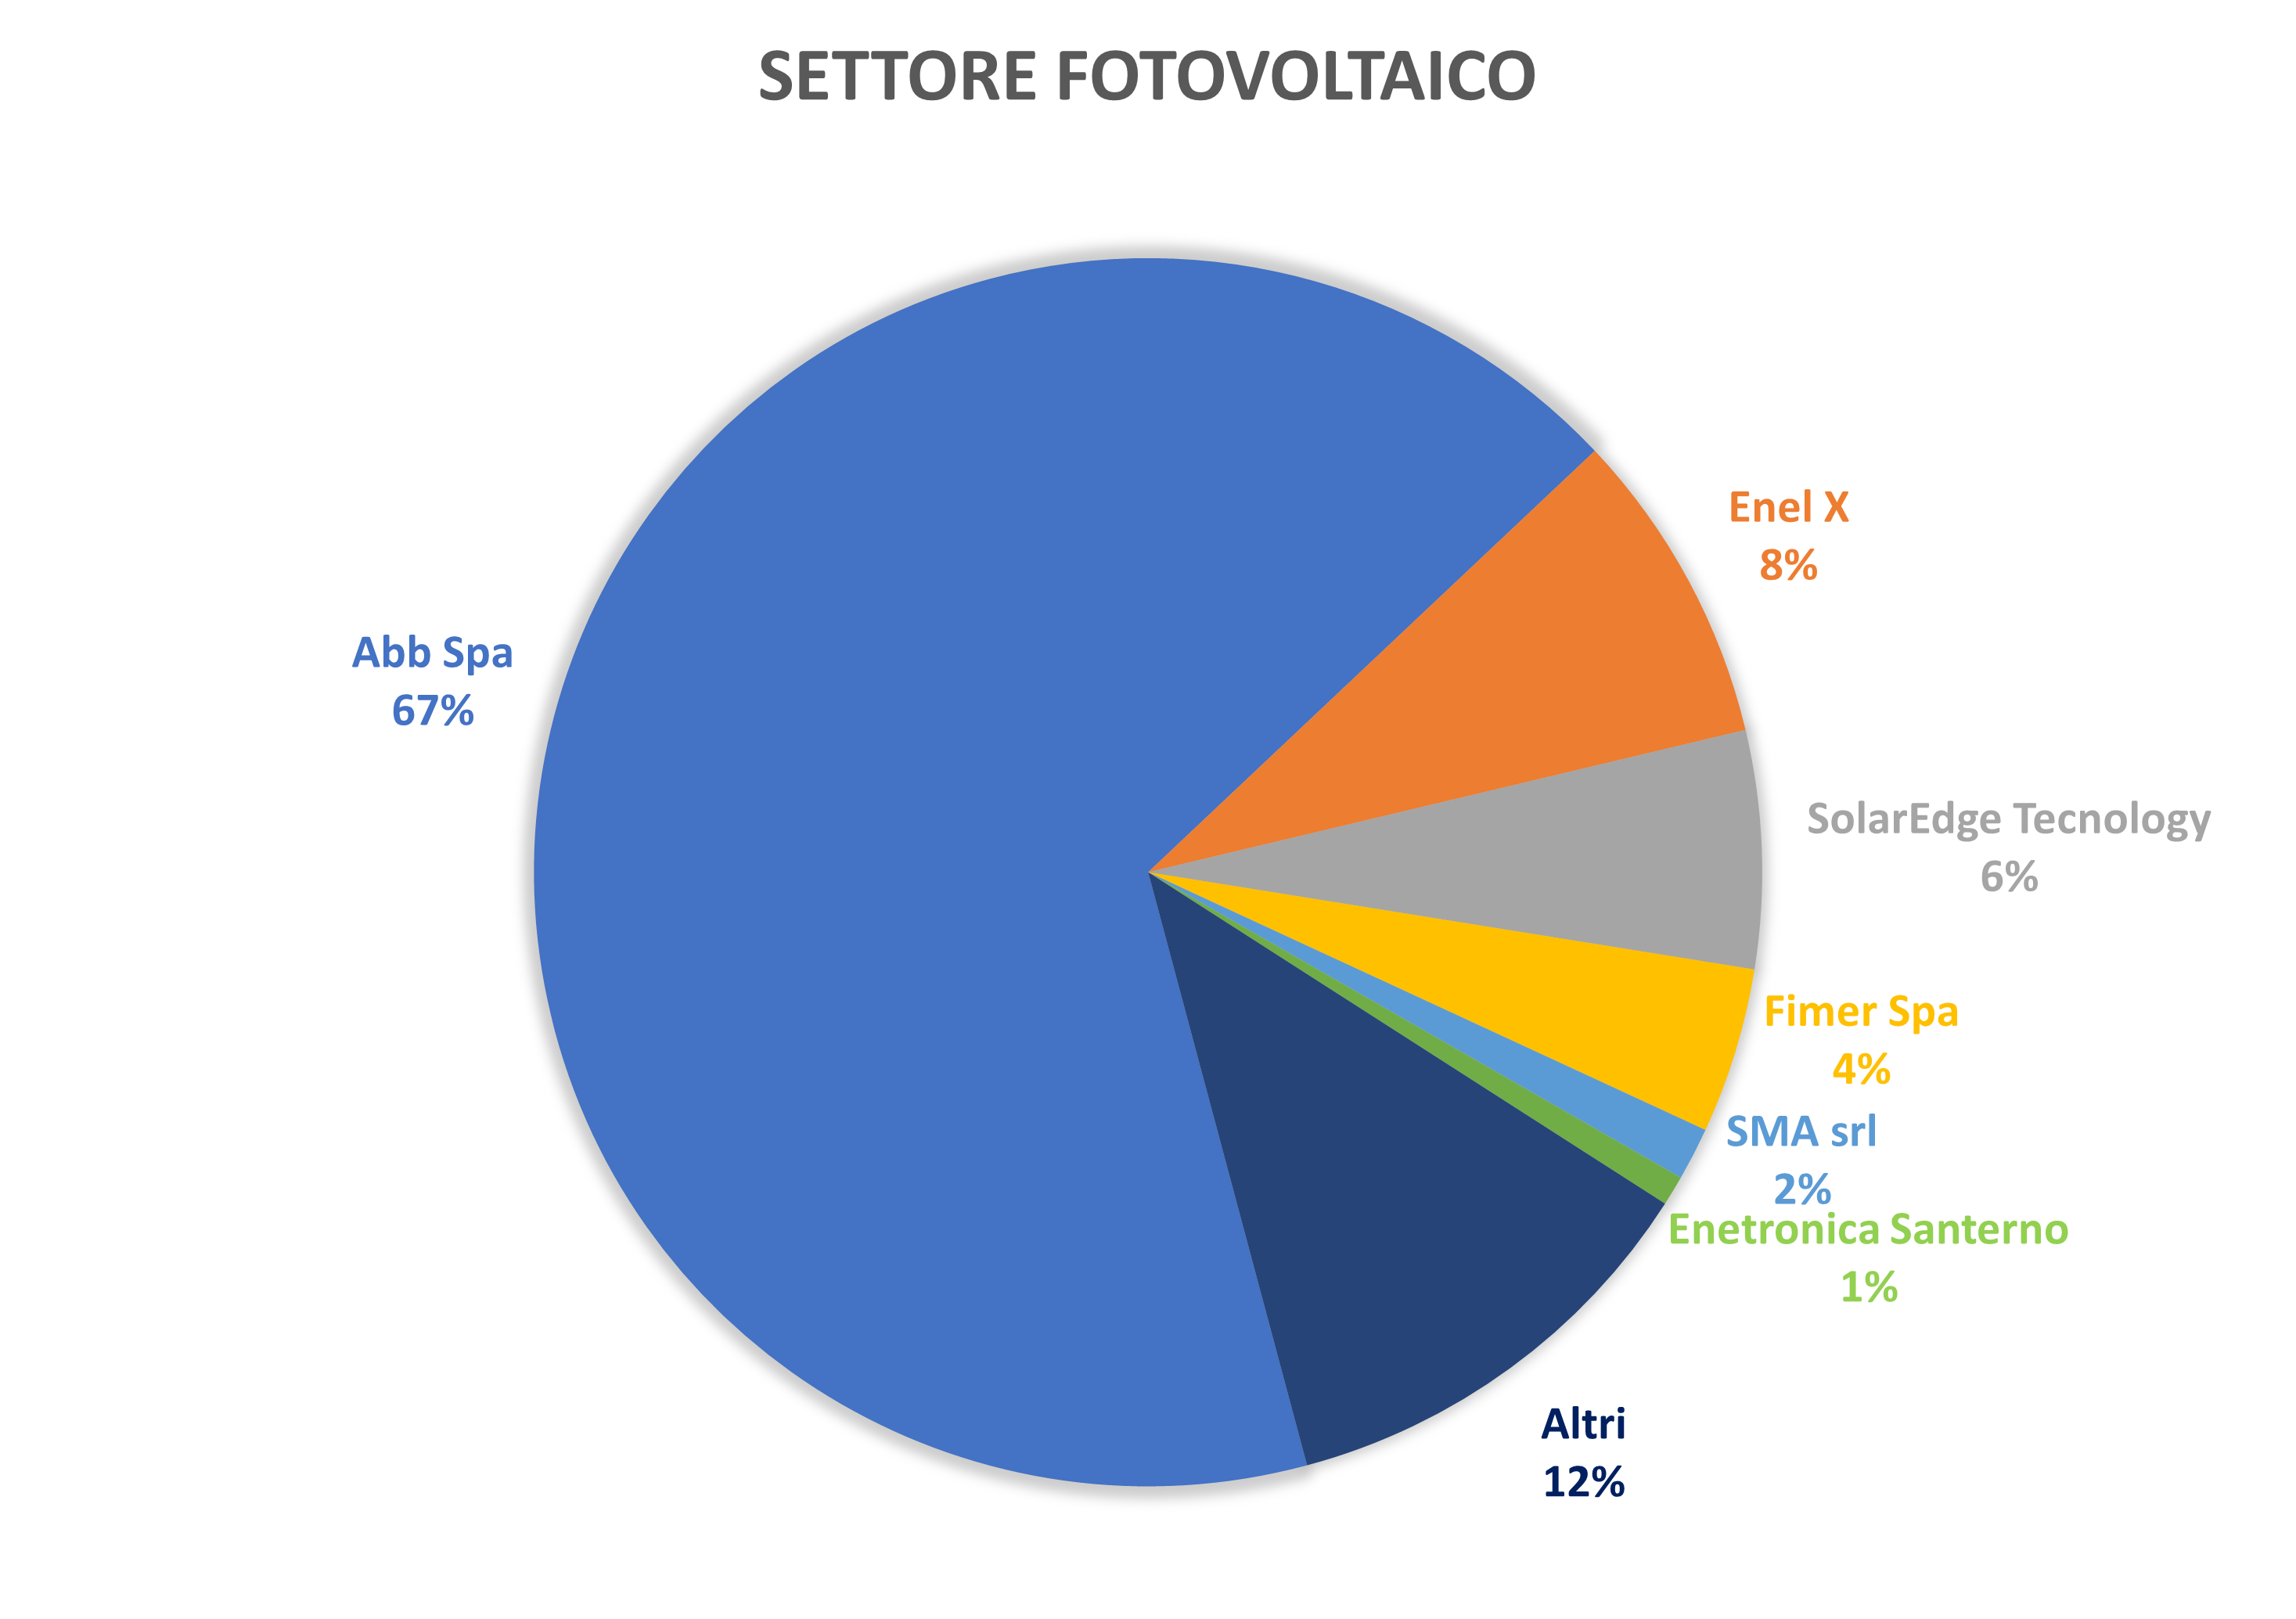
\includegraphics[width=0.7\textwidth]{Images/suddivisione_settore.png}
	\end{center}
	La proposta di \emph{Osmos} è ritenuta interessante per attuale situazione del settore, sia perché l'ambito del fotovoltaico si sta ampliando, sia a causa della mancanza di una soluzione a supporto dei moduli fotovoltaici specializzata nella pulizia di questi. La strategia adottata è riportata di seguito:
	\begin{center}
		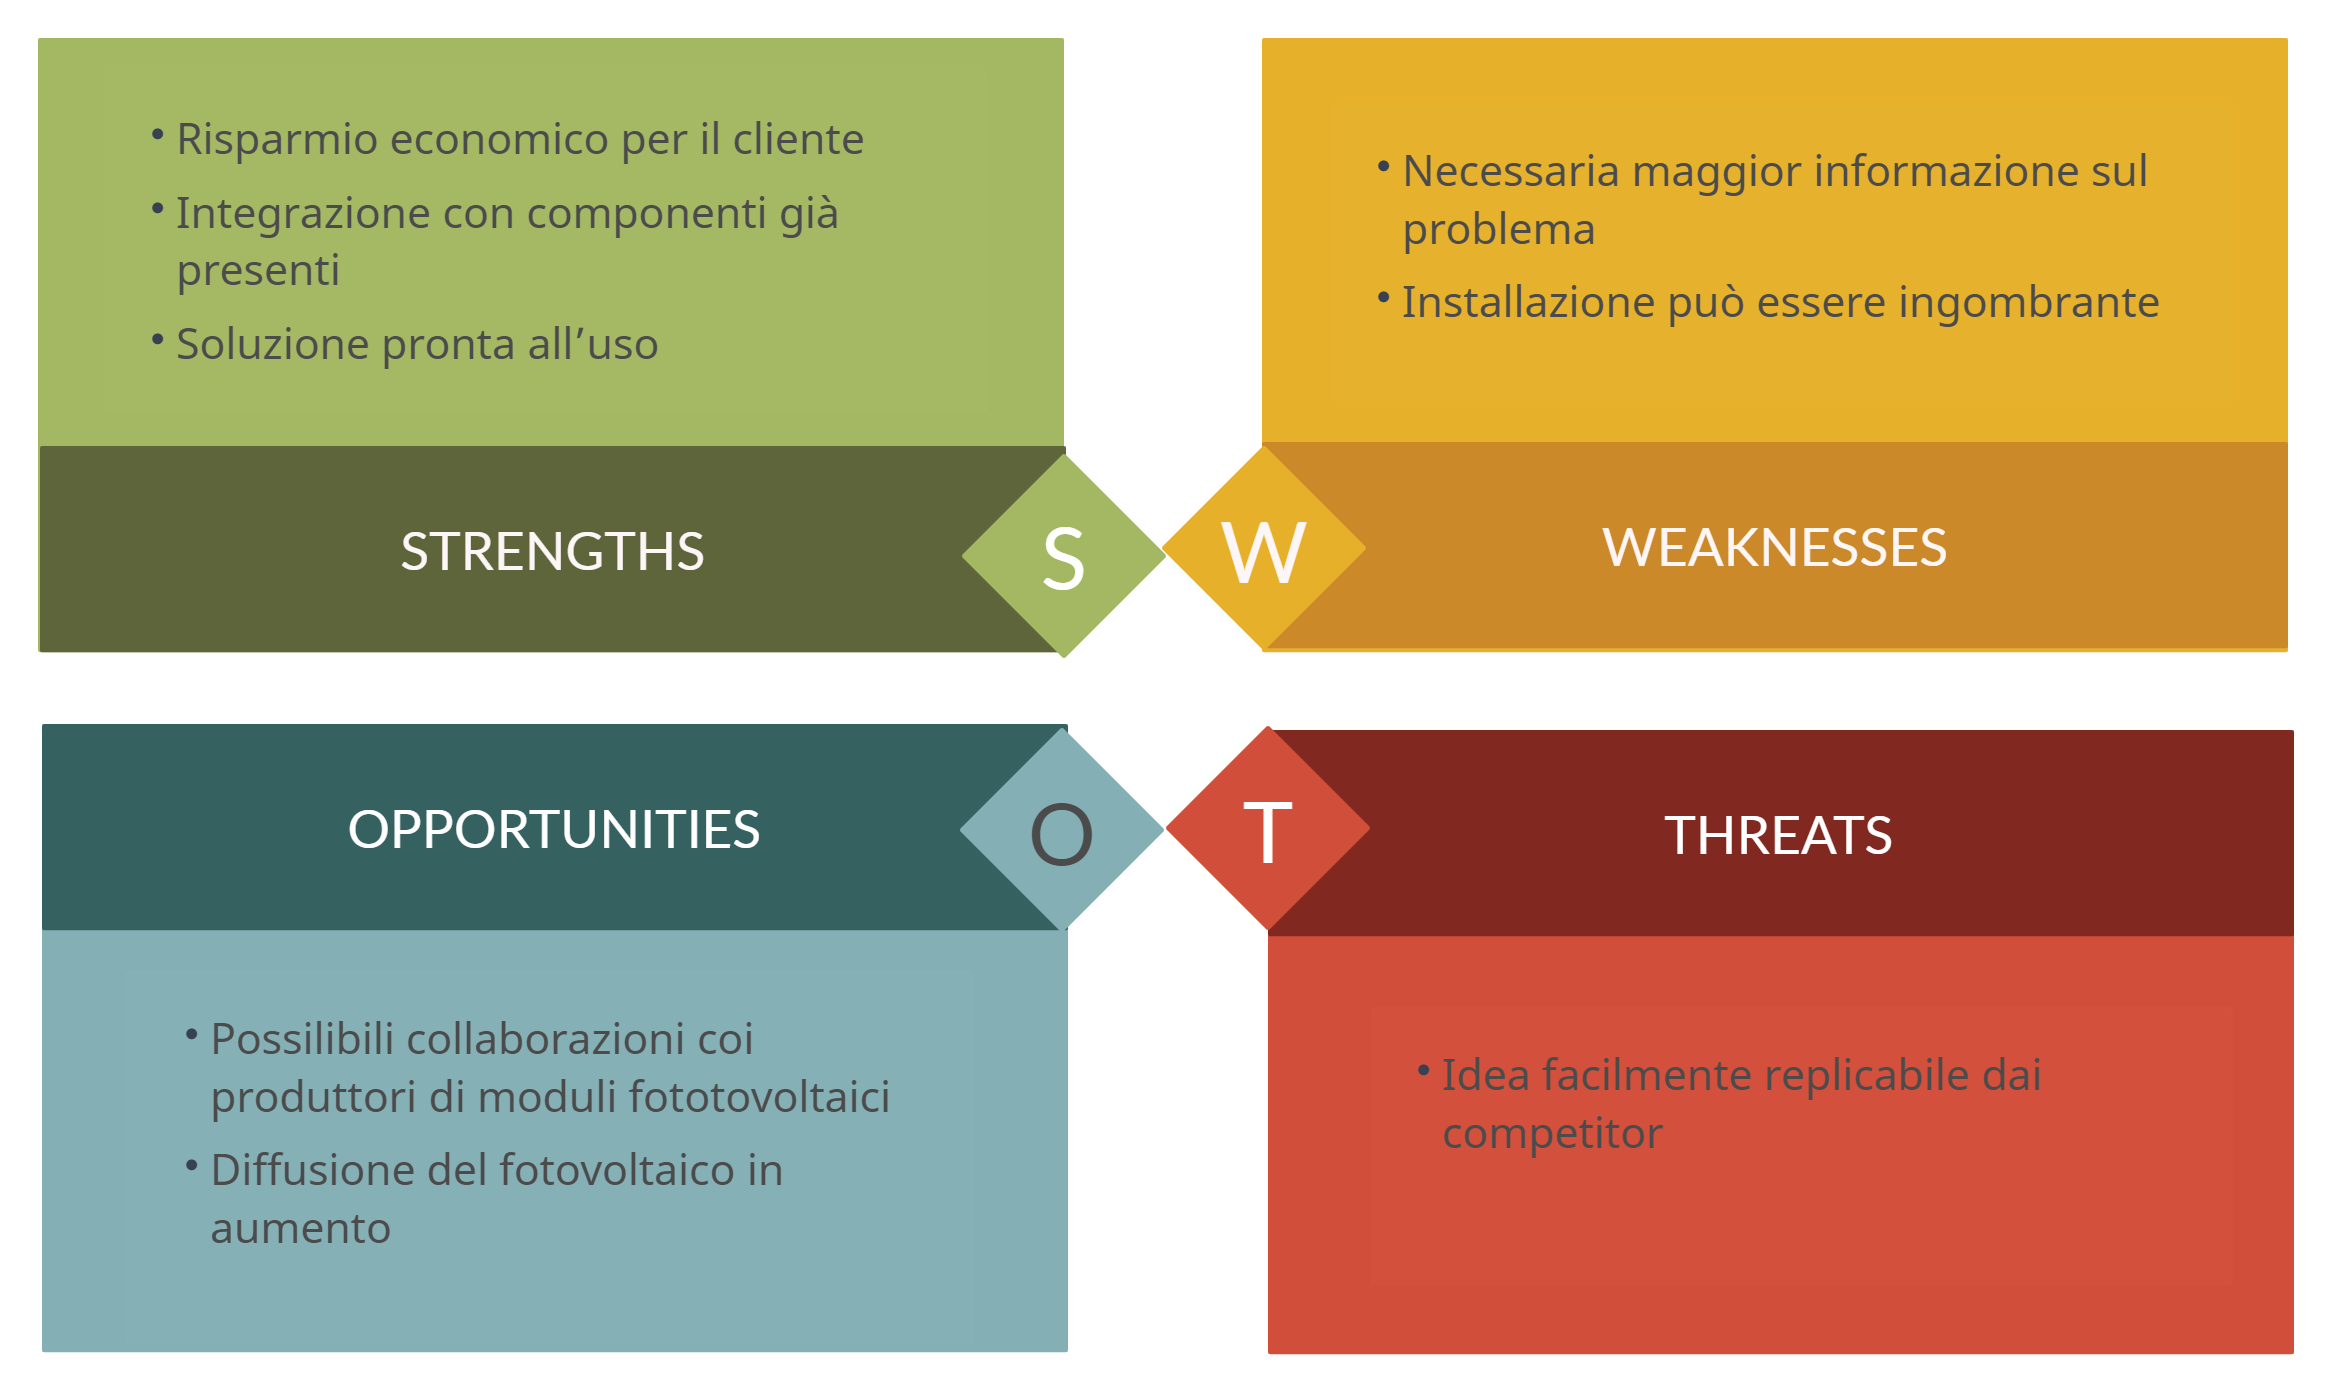
\includegraphics[width=0.65\textwidth]{Images/SWOT2.png}%\vspace{-2cm}
	\end{center}
	Oltre a ciò, si riportano qui gli obiettivi perseguiti da \emph{Osmos} confrontati con quelli dei principali competitor sopra citati:
	\begin{center}
		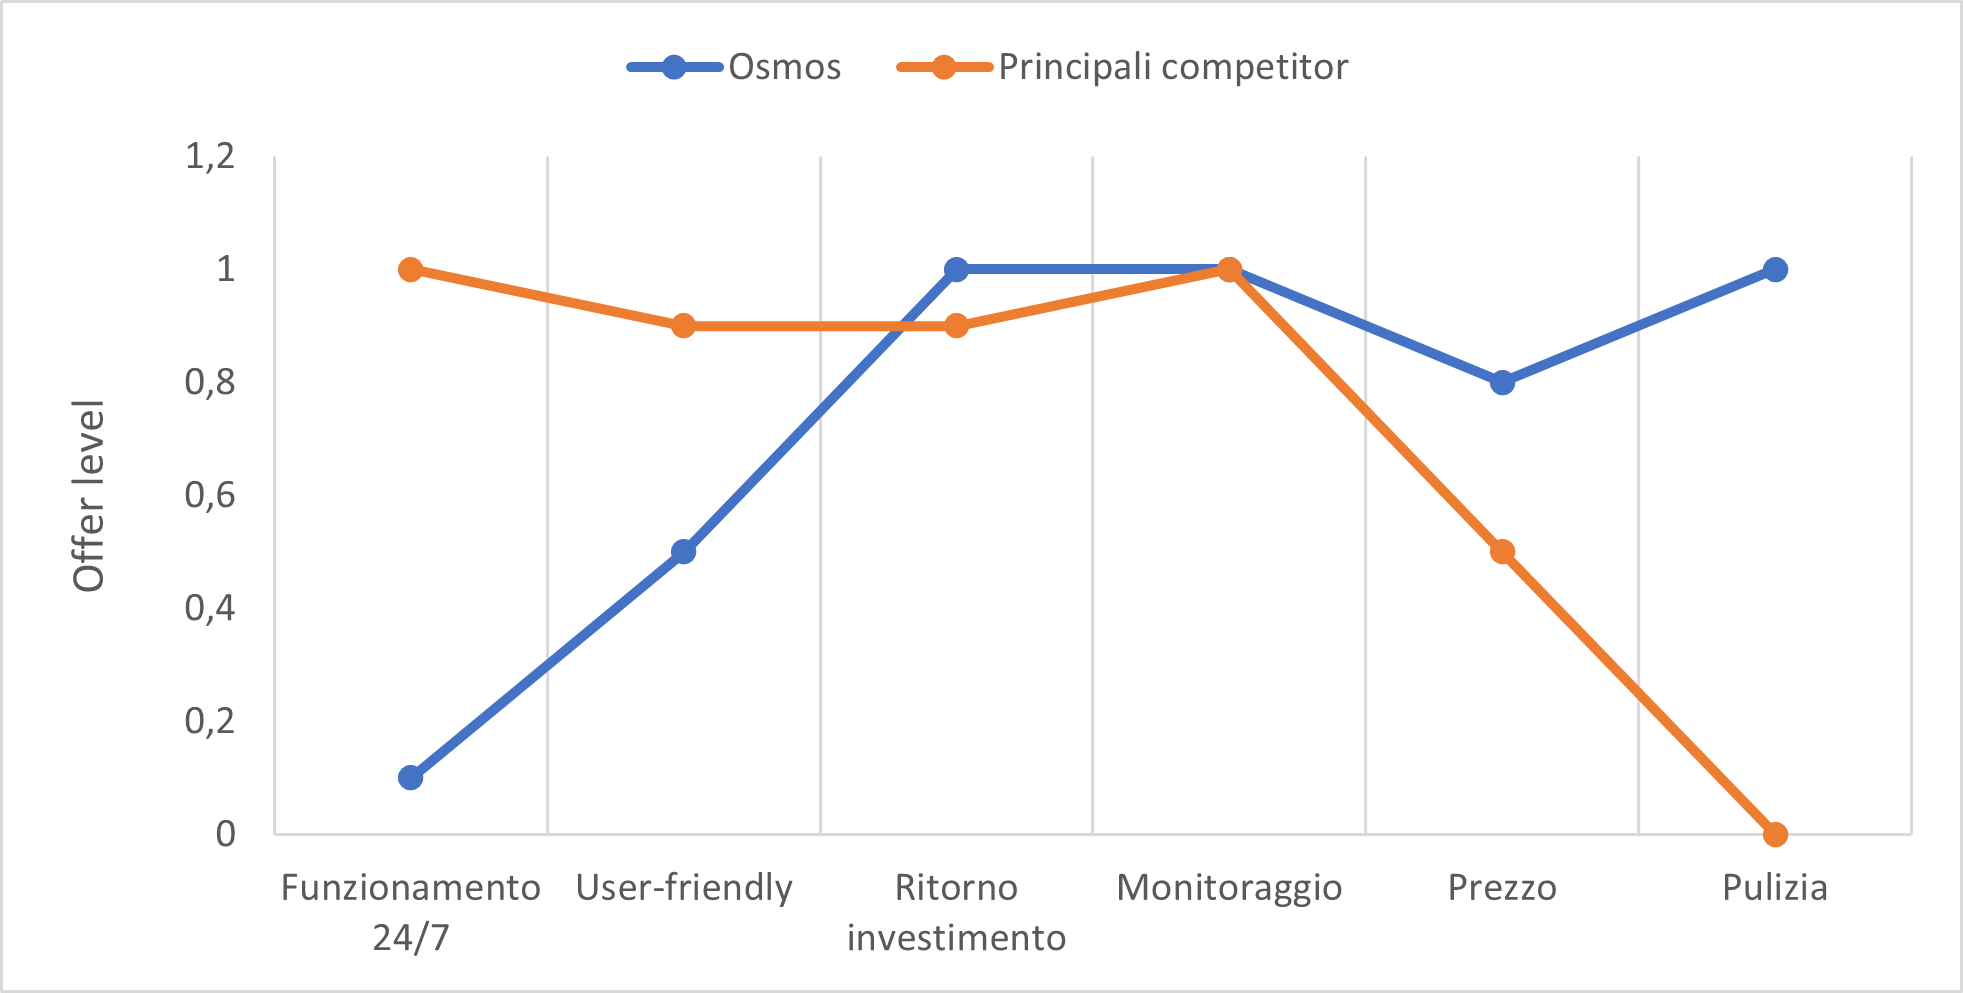
\includegraphics[width=0.8\textwidth]{Images/curve_valore.png}%\vspace{-2cm}
	\end{center}
	\section{Il mercato e il cliente}
	\section{Modello di business}
	\textbf{Value Proposition}\\
	L'obiettivo di \emph{Osmos} è fornire e installare sistemi per la pulizia automatica dei moduli fotovoltaici. Questi sistemi sono indirizzati sia agli utenti privati, possessori di impianti domestici, sia verso imprese che possiedono una superficie fotovoltaica notevolmente superiore. I sistemi proposti forniscono ai clienti non solo la possibilità di sfruttare impianti che mantengono un alto livello di efficienza energetica ma anche di risparmiare sul costo della pulizia, dal momento che non ci sarà più la necessità di rivolgersi ad una ditta esterna per eseguirla.\\
	Così facendo il cliente dovrebbe unicamente occuparsi di rifornirsi di acqua osmotica per riempire il relativo serbatoio con cui poi il sistema effettua la pulizia.\\\\
	\textbf{Relazione col cliente}\\
	Il primo contatto con il cliente può essere stabilito tramite la stessa impresa produttrice e installatrice dell'impianto fotovoltaico che informa della possibile installazione anche di un sistema \emph{Osmos}, oppure tramite spot pubblicitari online attraverso social network e pubblicità mirata. In questo modo diventa possibile intercettare anche e soprattutto consumatori entranti nel settore sempre crescente del fotovoltaico, rendendoli consci del problema fin dal momento dell'acquisto dei pannelli.\\
	Una volta entrati in contatto con l'acquirente, dopo l'avvenuta installazione si ha l'obiettivo di mantenere il rapporto col cliente tramite la fornitura di un servizio di assistenza disponibile per via telefonica, utilizzabile dall'utente per contattare l'assistenza in caso di malfunzionamenti del sistema o problemi di qualsiasi genere legati ad esso, di modo da poter intervenire tempestivamente.\\\\
	\textbf{Elementi chiave}\\
	\emph{Osmos} attribuisce molto peso all'esecuzione di un sopralluogo del sito di installazione per essere in grado di pianificare la soluzione che meglio si adatta al singolo cliente.\\
	Una volta avvenuta l'installazione risulta di vitale importanza un adeguato monitoraggio dell'efficienza energetica nel tempo, reso possibile dalla storyline dell'impianto fotovoltaico. Questa garantisce l'avvio della pulizia nel momento ideale allo scopo di attestare le prestazioni su valori elevati e di prolungare la vita del modulo fotovoltaico.\\
	Notevole importanza è poi attribuita anche ai partner. Come visto in precedenza, si ha intenzione di instaurare un legame con un'impresa fornitrice di impianti fotovoltaici. Questo garantirebbe non solo una più facile divulgazione dell'importanza della pulizia dei pannelli, ma andrebbe anche a favorire un aumento del numero di clienti entranti nel settore.\\ % si capisco il senso dell'ultima frase?
	Inoltre, avendo la possibilità di stipulare contratti con le imprese fornitrici di materie prime (quali piattaforme Arduino e componenti idraulici) si andrebbero a ridurre i costi di produzione, aumentando di conseguenza il margine di profitto.\\\\
	% idee:
	%	- adeguata pianificazione dell'installazione nel domicilio: soluzione applicata ad hoc per il cliente (attività)
	%	- collaborazione con impresa che installa pannelli (partner chiave) grazie ad essa si facilità la divulgazione del prblema che andiamo a risolvere
	%	- forniori di materie prime sia Arduino che a livello idraulico (partner)
	\textbf{Analisi costi e ricavi}\\
	In Italia, il costo medio per effettuare una pulizia completa dell'impianto si aggira tra i 100 e i 300\euro: un costo che varia a seconda della condizione in cui versano pannelli, della posizione di installazione di questi e dalle dimensioni della superficie. \emph{Osmos} punta a fornire un prodotto dal costo complessivo e indicativo per il cliente finale di 500\euro: un prezzo dato in gran parte dalla manodopera in fase di installazione ma variabile proprio in base a questa.\\
	Il costo delle materie prime è invece più limitato: oltre al software necessario (di nostra produzione) è richiesto solamente un modulo Arduino e le componenti idrauliche, per un costo totale stimato di 120\euro.\\
	L'obiettivo risulta quello di ottenere un profitto del 20\% su ogni installazione.
	\begin{center}
		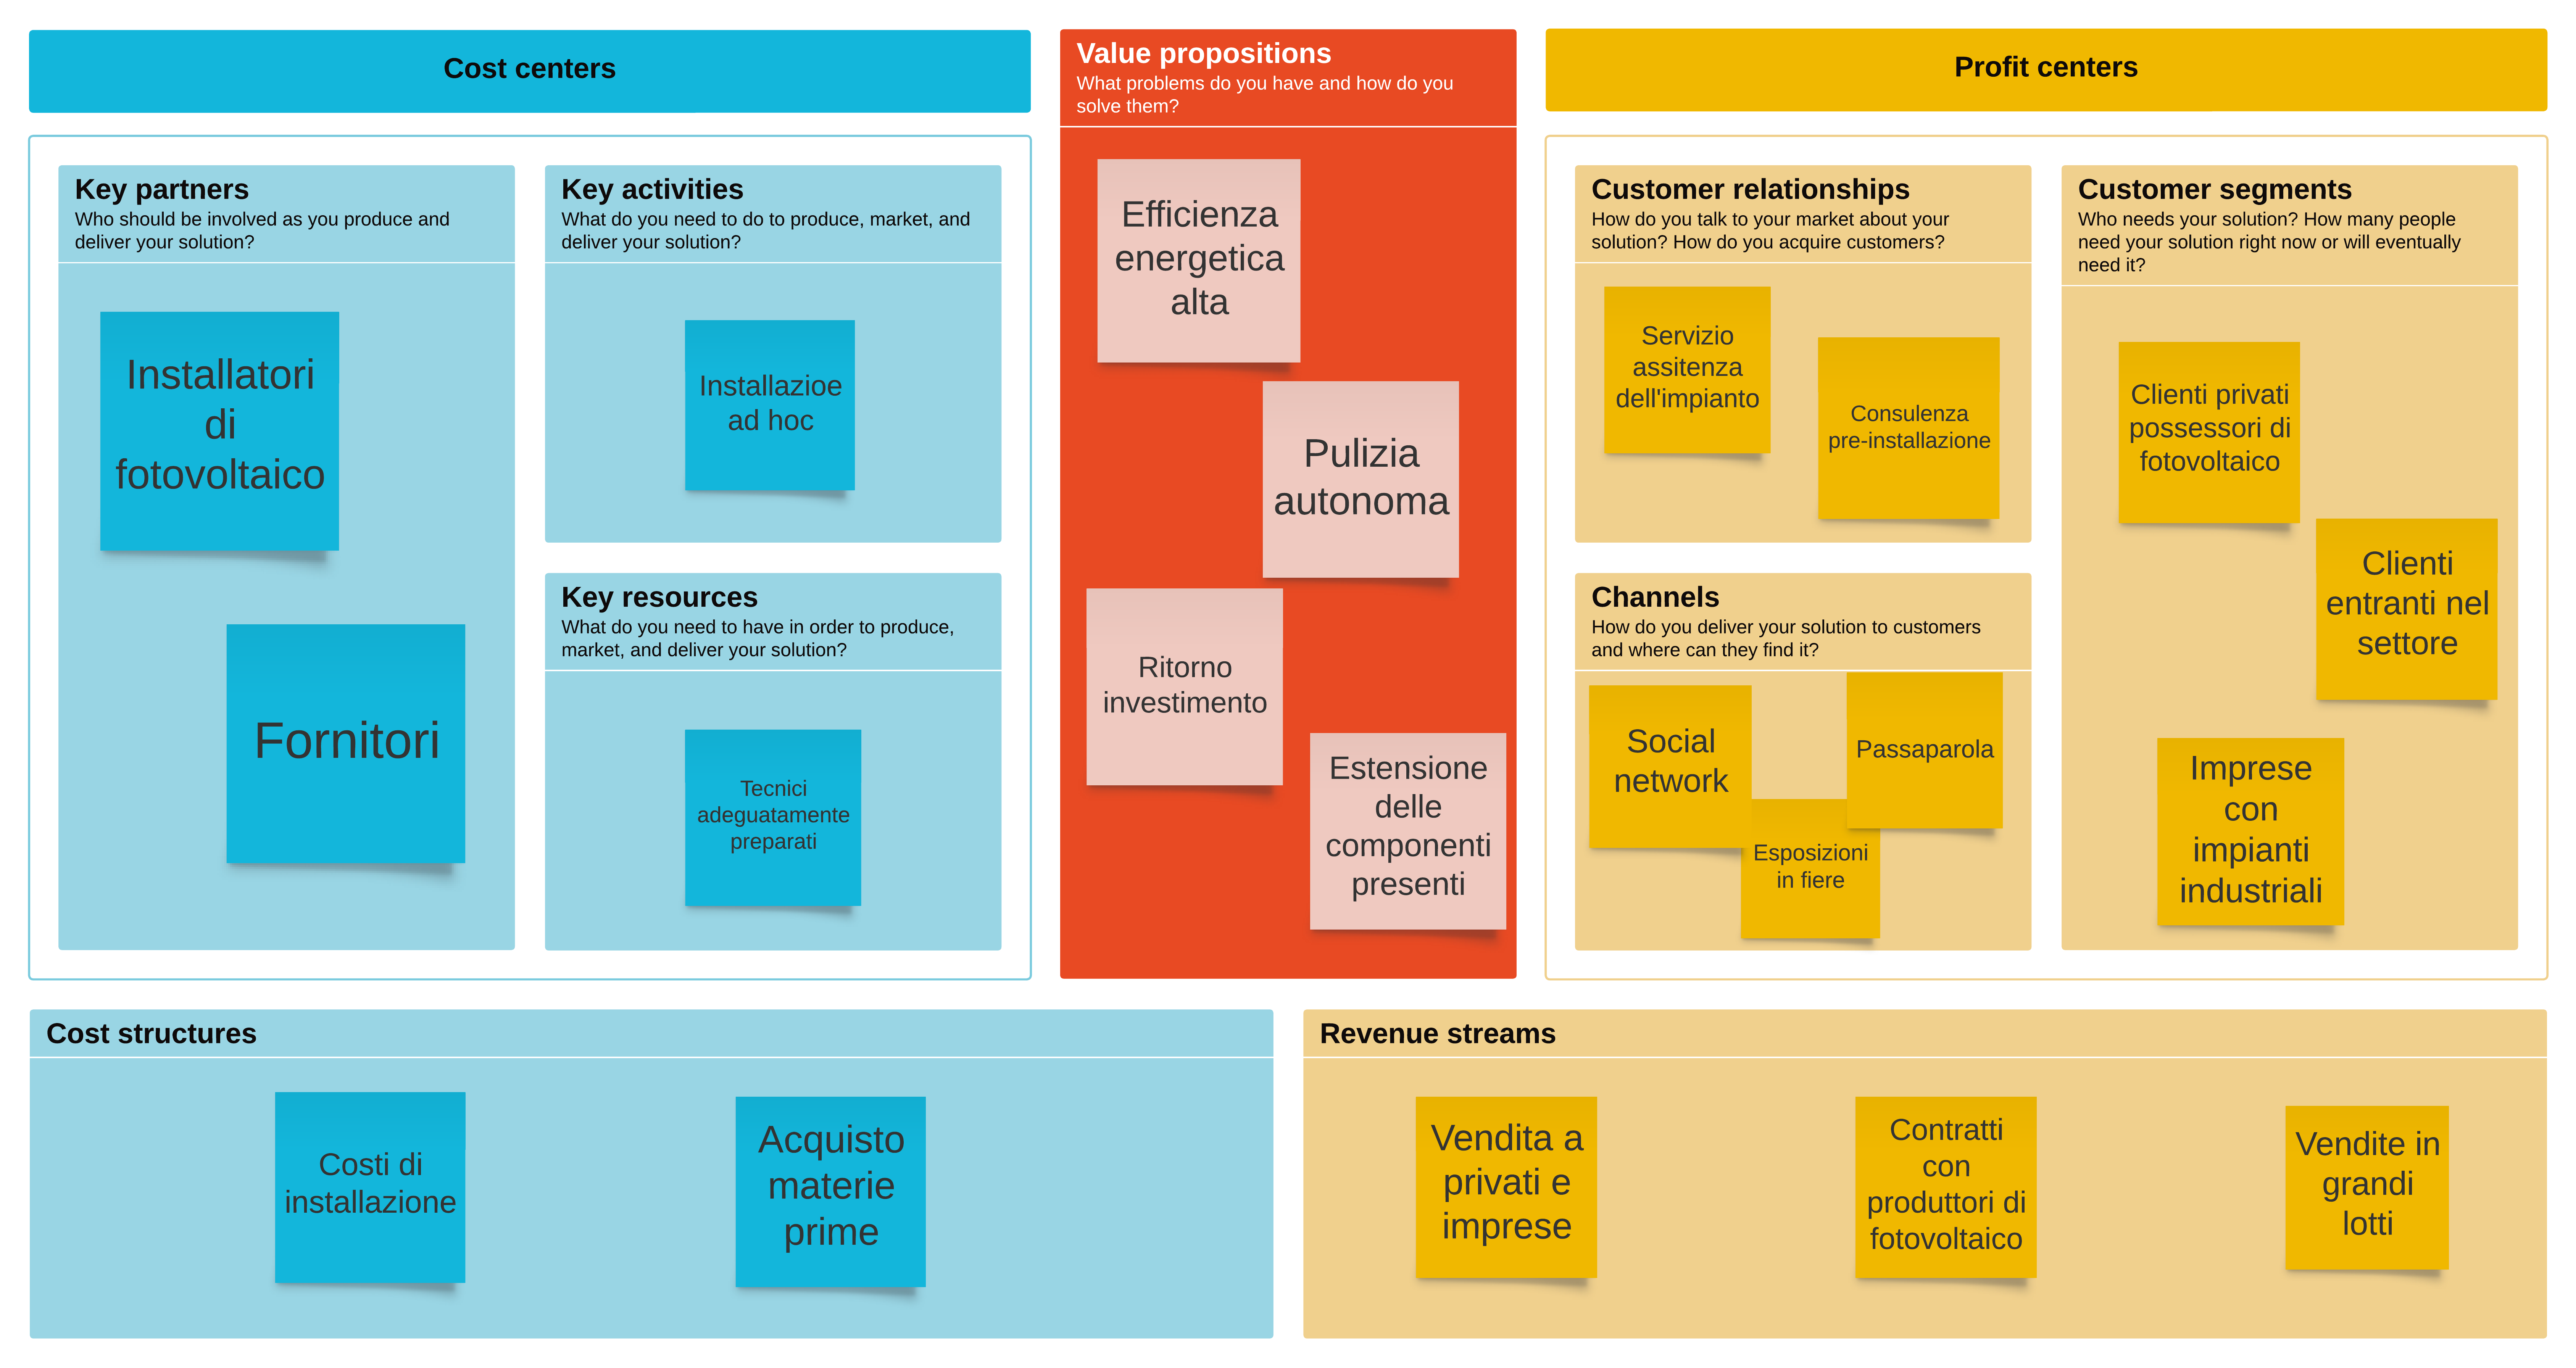
\includegraphics[width=0.9\textwidth]{Images/BusinessModelCanvas.png}
	\end{center}
	% idee:
	%	- esprimere il costo di una tradizionale pulizia, il nostro prodotto avrà un costo circa pari a quello della singola pulizia ma consentirà al cliente di non pacgare più per altri interventi
	%	- costi: manodopera per installazione (dipende da installazione a installazione) e materie prime... diciamo un 50 euro + manodopera?
	%	- prezzo di vendita = costi + 25%?
	\section{Funzionamento del prodotto}
	\begin{center}
		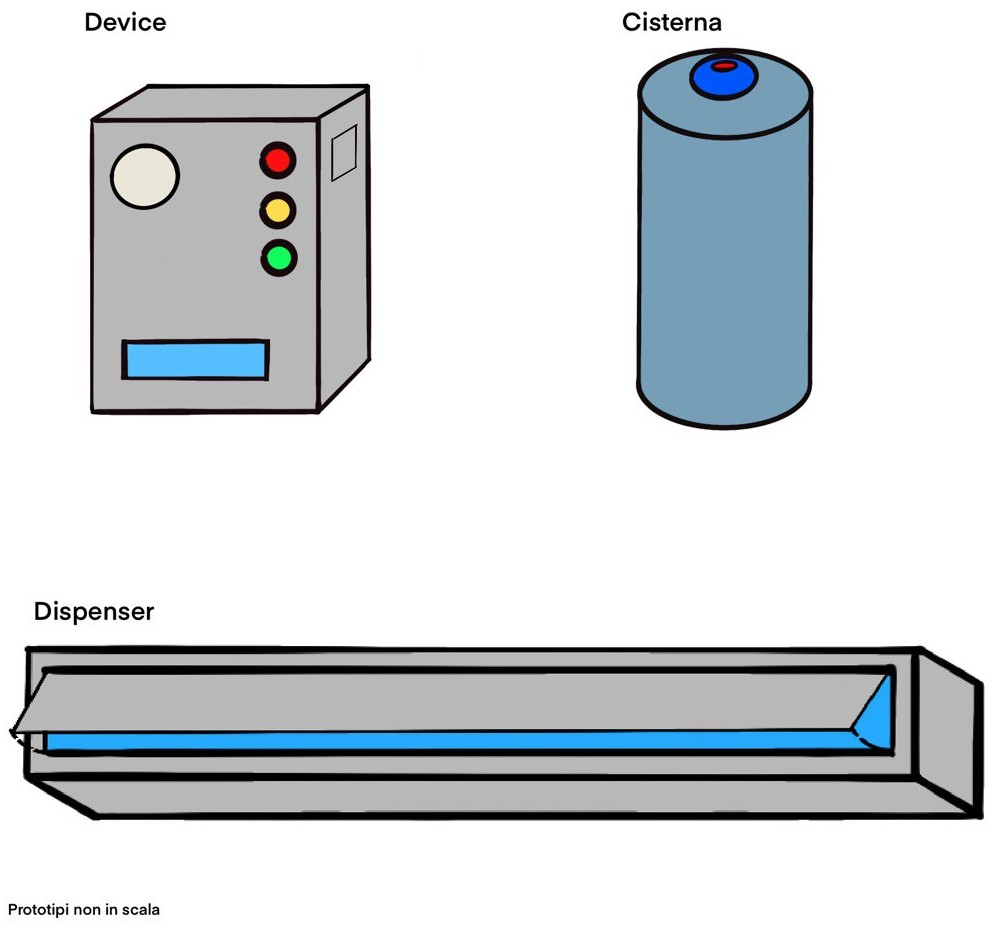
\includegraphics[width=0.5\textwidth]{Images/prototipo.jpg}
	\end{center}
	\section{WBS e Prospetto di Gantt}
	\begin{center}
		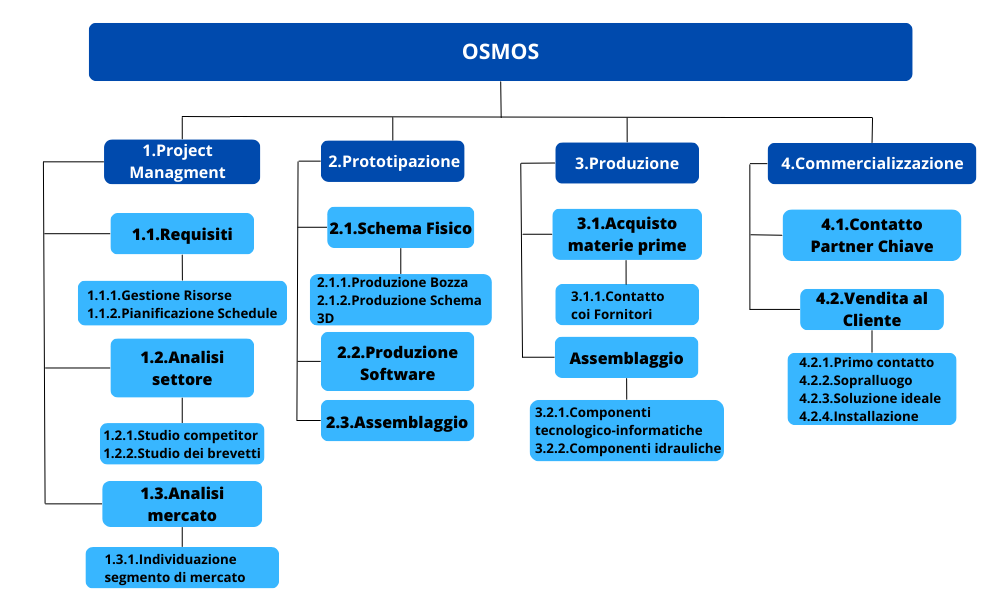
\includegraphics[width=0.9\textwidth]{Images/WBS.png}
	\end{center}
\end{document} 
